\svnkwsave{$RepoFile: siminos/baroclinic/intro.tex $}
\svnidlong {$HeadURL$}
{$LastChangedDate$}
{$LastChangedRevision$} {$LastChangedBy$}
\svnid{$Id$}

\chapter{Baroclinic flows}
\label{chap:baroclinic}

\section{Introduction}
\label{s:intro}
    \SOA{Not really sure if it is the hardest one to understand. But I
    remembered it seem to distant to me the first time the concept was
    introduced to me.}
The concept of baroclinic instability is perhaps one of the harder ones
to grasp in geophysical fluid mechanics. However, it is also one of the
most fundamental concepts on this field, as it is the main driver for the
large scale circulation of both the atmosphere and the ocean. It is by this
mechanism that the atmosphere redistributes heat from low latitudes to
high latitudes, that it sustains synoptic weather systems, and by which
some oceanic eddies are develop. Its importance can not be
overstated.

    \SOA{Here I am mostly speculating. However, this is the impression I
    have so far}
On the other hand, one could argue that the study of baroclinic flows
remains in its early stages. Although there exist a very well developed
linear theory for the onset of this type of instability, there still much
room to explore the nonlinear regimes. A way to approach this studies is
given by recent advances in the theory of nonlinear systems (some
references); making use of the symmetries of the system, and finding
periodic orbits and fixed points, as a way to understand the manifold of
this type of setups.

In this study we introduce the physics and present the nonlinear theory
methods that might be used to analyze baroclinic flows. We will briefly
mention some of the stability theory, but the emphasis would not be on
them. Great papers have been written about it an the reader is referred
to references [.....].

The work is divided as follows. In \refsect{s:examples} we introduce the
problem in a qualitative matter, hopping that this simple approach gives
away the underlying physical principle. In \refsect{s:vorticity} we
use Navier-Stokes equation to derive the vorticity equation and
explicitly expose the term which contribute to this instability (i.e. the
solenoidal term); we also show how can this induce circulation in the
simple setups given in \refsect{s:examples}. In \refsect{s:qg} we
introduce the QG-Equations, which are a simplified set of equations
suitable to study geophysical flows. We also present simulations for the
case were a two layer model is considered.  \refSect{s:stability}
introduces some basic setup showing how the stability of this flows might
be addressed. An we devote the remainder of this work in showing how
nonlinear techniques can be used to identify important properties of this
types of flows.

\section{Qualitative Examples}
\label{s:examples}
\SOA{Just a rough draft at this time, would continue to work soon.}
There are plenty examples which illustrate the mechanism initiating baroclinic flows, however let us start with the simpler ones, and we will progressively built up in complication. To start with, let us ignore the effects due to earths rotation and concentrate only in inertial frames. That is, let's start not by treating baroclinic instability perse, but the process by which a fluid adjust to equilibrium given a uneven distribution in density. A great example of this is Marsigli's experiment to explain undercurrent flows in the Bosphorus river from the Mediterranean to the Black Sea (see \refref{Gill82}), and we will begin with a mental experiment based on this.

Consider the situation shown in Figure \ref{f:drivedrag}.a, where two fluids of different densities, initially separated at $x_o$, are suddenly allowed to interact. The situation is clearly unstable; a pressure gradient would exist at all levels, except for the surface, going from the heavier fluid to thee lighter one. This would create both subsurface and surface currents, one due to the pressure gradient in the bottom, and the other due to mass conservation in the surface. Intuitively we can imagine that the system would finally settle to a configuration where the heavier fluid would lay on the bottom and the lighter one on top. That is, a configuration where the potential energy is minimized.

Thinking about this problem in terms of surface of constant pressure and density we can understand the instability that causes this type of behavior. In the initial configuration, the isopycnals are orthogonal to the isobars Figure \ref{f:drivedrag}.b, so that the mentioned pressure gradient is generated at $x_o$. Later, as the denser fluid starts to settle in the lower layer, this pressure gradient starts to spread out; but it will always exist as long as there is a inclination is the isopycnals. At the end, when all the transient motions are settled and equilibrium is reached, both  the isobars and the isopycnals are parallel; leaving the system in a lower potential energy state. A fundamental concept can be extracted from this: 

\emph{In the absence of rotation, and an external forcing, equilibrium of a fluid is reached when isopycnals and isobars are parallel to each other}. 

If this condition is not met, transient motions would be generated to extract the excess  potential energy, and leave the system in its lower energy state.

%%%%%%%%%%%%%%%%%%%%%%%%%%%%%%%%%%%%%%%%%%%%%%%%%%%%%%%%%%%%%%%%
\begin{figure}[t]
\begin{center}
 \begin{tabular}{cc}
        ~~~~~~~~(\textit{a})                        &   ~~~~~~~~(\textit{b}) \\
    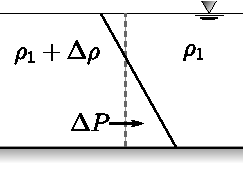
\includegraphics[width=0.46\textwidth, clip=true]{inertialAdjustment}
    & 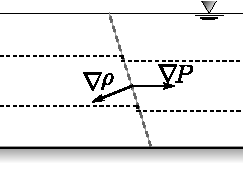
\includegraphics[width=0.46\textwidth, clip=true]{inertialAdjustmentb}

  \end{tabular}
\end{center}
\caption{
(a) Adjustment of a fluid subject to a horizontal difference in density in a non-rotating frame.
(b) Isopycnals and isobars(dashed lines), and the pressure and density gradient for a unstable condition.
        }
\label{f:drivedrag}
\end{figure}
%%% INCLUDE A FIGURE HERE  \ref{f:Marsigli}
%%%%%%%%%%%%%%%%%%%%%%%%%%%%%%%%%%%%%%%%%%%%%%%%%%%%%%%%%%%%%%%%%

The term responsible for the instability is quantified mathematically as the curl between the density and pressure gradients, that is:

\beq
\nabla \rho \times \nabla p
\ee{solenoid}

as we will show in \refsect{s:vorticity}. Obviously, this definition
agrees with the intuitively notion we just developed.

Consider now a further complication, and think about what would happen if
the frame of reference were to be rotating in our previous experiment. In
that case we would have to consider the apparent forces that develop on
the individual fluid parcels of our flow, one proportional to the
position (the centrifugal acceleration) and other proportional to the
velocity (the Coriolis force) of each parcel. However, in geophysical
applications the former one is unimportant\rf{Holton79}, and only the
effects of the Coriolis Force needs to be consider. Thus, if we repeat
our experiment from a initial state as before, the motion of the fluid
would be determined by the effects of the pressure gradient and the
Coriolis force.

In this new setup, each individual parcel starts moving due to the
pressure gradient force but the presence of rotation makes them deviate
from a straight trajectory; this because Coriolis force acts at right
angles of the parcel velocity. After these transient motions have
disappear, an new balance state is reached, where the velocity becomes
perpendicular to the pressure gradient force (see \reffig{f:GBalance}).
This balance state is referred commonly as geostrophic balance, and it
differs from the previous example in that in this new balance the
pressure gradient does not vanishes, but rather is balanced by the
Coriolis force. That is, from the inviscid, unforced Navier-Stokes
equations one would get:
\beq
\textbf{u}_g=-\frac{1}{f \rho} \textbf{k} \times \nabla_z p
\ee{Geostrophic}
where $\textbf{u}_g$ is the horizontal component of the velocity, $f$ is
the Coriolis parameter, $\rho$ is the density of the flow, $p$ is the
pressure and $g$ the acceleration due to gravity. In addition, the use of
the hydrostatic relation implies the following relation for the change in
the vertical; which is commonly referred as the thermal wind equation\rf{Salmon98}:
\beq
\frac{\partial \rho u_g}{\partial p} =\frac{1}{f} \left(\frac{\partial \alpha}{\partial y}\right)
\ee{TWE1}
\beq
\frac{\partial \rho u_g}{\partial p} =-\frac{1}{f} \left(\frac{\partial \alpha}{\partial x}\right)
\ee{TWE2}

where $\alpha$ is the specific volume of the fluid.
%%%%%%%%%%%%%%%%%%%%%%%%%%%%%%%%%%%%%%%%%%%%%%%%%%%%%%%%%%%%%%%%
\begin{figure}
\begin{center}
  % Requires \usepackage{graphicx}
  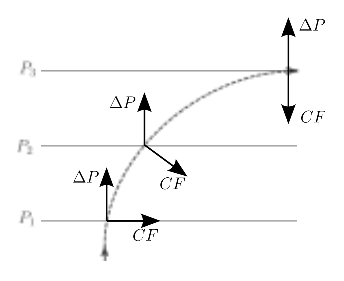
\includegraphics[width=0.5\textwidth, clip=true]{GeostrophicBalance}\\
\end{center}
  \caption{Process of geostrophic adjustment for an initially motionless fluid parcel.}
  \label{f:GBalance}
\end{figure}
%%% INCLUDE A FIGURE HERE  \ref{f:GBalance)
%%%%%%%%%%%%%%%%%%%%%%%%%%%%%%%%%%%%%%%%%%%%%%%%%%%%%%%%%%%%%%%%%

From the last relations, we conclude that there is a equilibrium state
that we can reach, in the presence of rotation, where the isopycnals and
isobars are not necessarily parallel to each other. Nonetheless,
instability occurs when the isopycnal slope exceeds a critical value;
this type of phenomena which is referred as baroclinic instability (see
\refref{Salmon98}).

It is left for the remainder of this work to inquire the stability
properties of this equilibrium, and the motions around it. The first of
this questions has been studied widely, and it uses linear approximations
to develop the relations between flow properties that need to be meet in
order for it to remain stable, or become unstable. The study of the motions that
develops after the initial instability is a more challenging problem as
nonlinear terms now become important, the hopes are that nonlinear theory
allow us to extract important knowledge about this phenomena.

\section{Vorticity Equation}
\label{s:vorticity}

What is clear from Marsigli's experiment, is that the impact of the
solenoidal term is to induce vorticity to the fluid\footnote{The reader
is referred to \refref{kundu08} for an introductory, yet rigorous
treatment of Vorticity. However, be aware that in his derivation of the
vorticity equation the density is not treated as a function of both
pressure and temperature, but only of pressure; so that the solenoidal
term is not considered.}. This last is a fundamental property of the
fluid, and studying it has the power of greatly simplify the analysis of a
given flow. In fact, the first satisfactory attempts to model the atmosphere
where done by Charney considering the vorticity of quasigeostrophic flows.

Vorticity arises naturally from Navier-Stokes equations, and is just
a measure of the rotational speed of the fluid parcel. To make the
derivation explicitly, let's consider the inviscid equations of motion in
a rotating frame of reference\footnote{As explained in Section
\ref{s:intro}, only the Coriolis' force ($\Omega \times \textbf{u}$) is
considered in the equations, as the centripetal acceleration due to
earths rotation can be ignored.}, that is:
\beq
\frac{\partial \textbf{u}}{\partial t}+(\textbf{u} \cdot \nabla)\textbf{u}+2\Omega \times \textbf{u} = -\frac{1}{\rho} \nabla p
\ee{NS1}
From vector calculus we note that:
\beq
(\textbf{u} \cdot \nabla)\textbf{u}=\frac{\nabla (\textbf{u} \cdot \textbf{u})}{2}- \textbf{u} \times \omega
\ee{VE0}
where $\omega$ is the vorticity. So that we can rewrite Navier-Stokes equation in the following way:
\beq
\frac{\partial \textbf{u}}{\partial t}+(\omega+2\Omega) \times \textbf{u} = -\frac{1}{\rho} \nabla p -\frac{\textbf{u} \cdot \textbf{u}}{2}
\ee{NS1}
Taking the curl of this equation (noting that $\omega = \nabla \times
\textbf{u}$) gives:
\beq
\frac{\partial \omega}{\partial t}+\nabla \times ((\omega+2\Omega) \times \textbf{u}) = -\nabla \times\left(\frac{1}{\rho} \nabla p\right) -\nabla \times \frac{\textbf{u} \cdot \textbf{u}}{2}
\ee{VE1}
Finally using use of the identity $\nabla \times (A \times B) = A (\nabla
\cdot B)-B (\nabla \cdot A)+(B \cdot \nabla)A-(A \cdot \nabla)B$, the
chain rule for the pressure $\frac{1}{\rho} \nabla p = \nabla (p/\rho)-p
\nabla (1/\rho)$, and the fact that the curl of a gradient is zero, the desired expression for the vorticity it is obtained from Equation \refeq{NS1} (see \refref{Salmon98} for further detail). That is:
\beq
\frac{d}{d t}\left(\frac{\omega_a}{\rho}\right)=\left[\left(\frac{\omega_a}{\rho}\right) \cdot \nabla \right] \textbf{u}+\nabla p \times \nabla \left(\frac{1}{\rho}\right)
\ee{VE2}
where $\omega_a=\omega+2\Omega$ is the absolute vorticity. It is then
evident from this equations how the baroclinic term ($\nabla p \times \nabla (1/\rho)$) can induce vorticity in the fluid by means of the instabilities previously discussed.

Equation \refeq{VE2} can also be written for a single layer shallow water system as (see \refref{Vallis06}):

\beq
\frac{d}{dt}\left(\frac{\eta + f}{h}\right)=0
\ee{SW1}

where $\eta$ is the vertical component of the vorticity, $h$ the instantaneous depth of the fluid, and the quantity conserved is referred as potential vorticity ($q=\eta + f/h$). A generalization to two or  more layers is straight forward (see \refrefs{Vallis06,phillips51}).  Simplified form of this
expression, filtering unimportant motions for the large scale circulations
is developed next for a two layer system. However, the equations are
still rich in dynamics as advection terms are retained for the horizontal
(so that a lot of interesting nonlinearities remains). Up to the date
there still much interesting features of this system to be studied.
    \SOA{I could include here a discussion about Kelvin circulation theorem,
    and how the baroclinic term would induce currents such as the sea breeze.
    However, I think I am extending a little to much in the basics. Hopefully
    this would make the project more readable.}




\section{2 Layer QG-Equations}
\label{s:qg}
If we intend to study baroclinic instability, we need to be able to
capture two basic properties of the flow (as shown in
\refsect{s:examples}): the nearly geostrophic motions of the fluid and its vertical
structure as given by Equations \refeq{TWE1} and \refeq{TWE2}. One of the simplest mathematical systems that would capture
this type of behavior \refref{phillips51}, is a quasigeostrophic set of equations discretized
for two vertical layers. A quick derivation is given here. For more in
depth derivations the  reader is referred to
\refrefs{Vallis06,Holton79,Salmon98,phillips51}.

Consider the situation in Figure \ref{f:twolayer}, where we have two layer of different densities, equal depths $H$, and the Rossby number is small enough so that we can use the quasi-geostrophic approximation. The potential vorticity of each layer can then be written as:
\beq
q_i=\frac{\eta_i+f}{h_i}
\ee{PV}
where $\eta_i$ is the relative vorticity of each layer, $f$ the planetary vorticity and $h_i$ distance between layers\footnote{We follow the derivation and the notation of \refref{Vallis06}}. As we learned, this property must be conserved by each layer, then:

\beq
\frac{d q_i}{dt}=\frac{d}{dt}\left(\frac{\eta_i+f}{h_i}\right) \simeq \frac{d}{dt}\left(f+\eta_i-f\frac{h_i'}{H_i}\right)=0
\ee{PVC}

where the approximation is only valid when Rossby number is small. $H_i$ is the unperturbed layer thickness, and $h_i'$ is the thickness perturbation for layer $i$. Now let us introduce the geostrophic equations to approximate the wind and the vorticity. From Equation \refeq{Geostrophic} we know that velocities only depend on the pressure, and if we assume our fluid as incompressible then this will depend only on the height of the interfaces. Which we can in turn can be related to $h_i$. That is, the height of the surfaces is given by:

\beq
\eta_o = h_1 + h_2 = h_1'+h_2'+2H
\ee{HS1}

\beq
\eta_1= h_2 = h_2' + H
\ee{HS2}

The pressure in the first layer is given by:

\beq
p = g \rho_1 (\eta_o-z)
\ee{Pre}

So that the horizontal gradient is:

\beq
\nabla p = g \rho_1 \nabla \eta_o = g \rho_1 ( \nabla h_1' + \nabla h_2' )
\ee{Pre1}

And with the exact same procedure it is found for the second layer:

\beq
\nabla p =  g \rho_1 ( \nabla h_1' + \nabla h_2' ) + g' \rho_1 \nabla h_2'
\ee{Pre2}

where $g'=(\rho_2-\rho_1)/\rho_1$ is the reduced gravity. The geostrophic condition then gives for the top layer:
\beq
u_g = -\frac{g}{f} \frac{\partial}{\partial y}(h_1'+h_2')
\ee{GEOS}
\beq
v_g = \frac{g}{f} \frac{\partial}{\partial x}(h_1'+h_2')
\ee{GEOS2}

and for the bottom layer:

\beq
u_g = -\frac{g}{f} \frac{\partial}{\partial y}(h_1'+h_2')-\frac{g'}{f} \frac{\partial h_2'}{\partial y}
\ee{GEOS3}
\beq
v_g = \frac{g}{f} \frac{\partial}{\partial x}(h_1'+h_2')+\frac{g'}{f} \frac{\partial h_2'}{\partial x}
\ee{GEOS4}

From the equations above, it is clear that the equations can be written in terms of a stream function for each layer, such that $u_i=-\partial \psi_i / \partial y$, $v_i=\partial \psi_i / \partial x$ and the vorticity is simply written as $\eta_i = \nabla ^2 \psi$. The stream functions being:

\beq
\psi _1 = \frac{g}{f} (h_1'+h_2')
\ee{SF1}

\beq
\psi _2= \frac{g}{f} (h_1'+h_2')+\frac{g' h_2'}{f}
\ee{SF2}

An expression for the potential vorticity of each layer in terms of the stream functions, is obtained if we use these in Equation \refeq{PVC}:

\beq
q_1=\beta y + \nabla^2 \psi_1 + \frac{f_o^2}{g'H}(\psi_2-\psi_1)-\frac{f_o^2}{gH}\psi_1
\ee{LE1}

\beq
q_2=\beta y + \nabla^2 \psi_2 + \frac{f_o^2}{g'H}(\psi_1-\psi_2)
\ee{LE2}

where the term $f_o^2 \psi_1/gH$ is much smaller and can be dropped from the equations. 

Note, that we now have a closed set of equation to solve. The equations above are only dependent on $\psi_1$ and $\psi_2$, and as they are the potential vorticity for each layer, they are exactly conserved ($d q_i/dt=0$). Nonetheless, it is convenient to nondimensionalize the variables; and we use the same scales as in \refref{Bracco03} for this purposes. That is, we use $U$ for the characteristic velocity of the flow, $L_R=(g'H)^{1/2}/f_o$ the internal Rossby deformation radius as the horizontal scale, and $L_R/U$ for the time scale. This way, Equations \refeq{LE1} and \refeq{LE2} transform to:

\beq
q_1^*=\beta^* y + \nabla^2 \psi_1^* + F(\psi^*_2-\psi^*_1)
\ee{LEND1}

\beq
q^*_2=\beta^* y + \nabla^2 \psi_2^* + F(\psi^*_1-\psi^*_2)
\ee{LEND2}

where $\beta^*=\beta U / L_R^2$ and $F=f_o^2 L_R^2 /(g'H) = 1$ \SOA{I am not really sure if these is set to one in the simulations, however it is in \refref{Bracco03}}. The superscript denotes a nondimensional variable and will be dropped hereafter, writing above equations as:

\beq
q_1=\beta y + \nabla^2 \psi_1 + F(\psi_2-\psi_1)
\ee{LEND1a}

\beq
q_2=\beta y + \nabla^2 \psi_2 + F(\psi_1-\psi_2)
\ee{LEND2b}

Lastly, it is also convenient to introduce some sort of dissipation in the system. Newtonian dissipation can be added easily by considering the conservation equations for $q_i$ as in \refref{Bracco03}, that is:

\beq
\frac{d q_i}{dt}=\frac{\partial q_i}{\partial t}+J(\psi_i,q_i)=\nu \nabla^4 \psi_i
\ee{Cons}

where $J(\psi,q)=\psi_x q_y - \psi_y q_x$ and $\nu$ is a nondimensional viscosity coefficient.

Equations \refeq{LEND1a} and \refeq{LEND2b} together with \refeq{Cons} constitute a closed set for $\psi_1$ and $\psi_2$, far more convenient than its dimensional form, as on these all term are scaled so that its magnitude is $O(1)$. We can now use this model as a simplified version to study baroclinic instability. However, note that nonlinear terms are retained, so that its dynamics still is rich and not fully understand up to date.
%We begin by considering Boussinesq approximation to Navier-Stokes
%equations. This arise when the density variations are small compared to
%the absolute value of itself (as is often found in the ocean), and the
%equations are simplified by only retaining the effects of the changes of
%density for the gravity terms (see \refref{Vallis06}). The equations are:

\section{Stability Theory}
\label{s:stability}

\section{Nonlinear Theory}
\label{s:nonlinear}
\section{Setup}
\label{s:setup}
